% ============================================================
% D58 --- PDL Framework
% Derivation of the SU(3) Gauge Structure from the
% PDL Axioms C1--C4: Completion of the Standard Model
% Gauge Group SU(3) x SU(2) x U(1)
%
% Author  : Cedric Laubscher
% Date    : June 2026
% Licence : CC BY 4.0
% ============================================================

\documentclass[11pt,a4paper]{article}

% ---- Encoding and language ---------------------------------
\usepackage[utf8]{inputenc}
\usepackage[T1]{fontenc}
\usepackage[british]{babel}
\usepackage{lmodern}
\usepackage{microtype}

% ---- Mathematics -------------------------------------------
\usepackage{amsmath,amssymb,amsthm}
\usepackage{mathtools}

% ---- Layout ------------------------------------------------
\usepackage{geometry}
\geometry{margin=2.5cm}
\usepackage{enumitem}
\usepackage{setspace}
\onehalfspacing
\usepackage{float}
\usepackage{booktabs}
\usepackage{longtable}
\usepackage{array}
\usepackage{xcolor}

% ---- Hyperlinks and metadata -------------------------------
\usepackage{hyperref}
\hypersetup{
  colorlinks=true,
  linkcolor=blue!60!black,
  citecolor=blue!60!black,
  urlcolor=blue!60!black,
  pdftitle={Derivation of the SU(3) Gauge Structure from the PDL Axioms C1--C4},
  pdfauthor={Cedric Laubscher}
}
% ---- PDF bookmark string sanitisation (PDL convention) -----
% Rule: every \section/\subsection title containing maths uses
% \texorpdfstring{$...$}{text version}. This block covers macros
% that may appear in bookmark contexts via running text.
\pdfstringdefDisableCommands{%
  \def\\{}%
  \def\Sfour{S4}%
  \def\Vfour{V4}%
  \def\Afour{A4}%
  \def\Sthree{S3}%
  \def\Zthree{Z3}%
  \def\SUthree{SU(3)}%
  \def\SUtwo{SU(2)}%
  \def\Uone{U(1)}%
  \def\PSUthree{PSU(3)}%
  \def\Kfour{K4}%
  \def\Re{Re}%
  \def\PDL{PDL}%
  \def\cong{=}%
  \def\times{x}%
  \def\setminus{ minus }%
  \def\subset{ subset }%
  \def\wedge{ and }%
  \def\_{-}%
  \def\Aut{Aut}%
  \def\Sym{Sym}%
  \def\Dic{Dic}%
  \def\GL{GL}%
  \def\RR{R}%
  \def\ZZ{Z}%
  \def\CC{C}%
  \def\FF{F}%
  \def\sinW{sin2W}%
  \def\thetaW{thetaW}%
  \def\suthree{su(3)}%
  \def\sutwo{su(2)}%
  \def\cartan{h}%
  \def\mathbb#1{#1}%
  \def\mathrm#1{#1}%
  \def\mathfrak#1{#1}%
  \def\mathbf#1{#1}%
  \def\textsc#1{#1}%
}

% ---- Bibliography ------------------------------------------
\usepackage[numbers]{natbib}

% ---- Tikz and tcolorbox ------------------------------------
\usepackage{tikz}
\usetikzlibrary{positioning,shapes.geometric,arrows.meta,fit,backgrounds,calc}
\usepackage{tikz-cd}
\usepackage{tcolorbox}
\tcbuselibrary{theorems,skins,breakable}

% ---- Colour palette (PDL convention) -----------------------
\definecolor{proofblue}{RGB}{0,70,140}
\definecolor{conjecturegreen}{RGB}{0,120,60}
\definecolor{openproblemred}{RGB}{160,20,20}
\definecolor{resolvedgreen}{RGB}{0,130,70}
\definecolor{chaincolor}{RGB}{30,100,180}
\definecolor{epscolor}{RGB}{160,60,0}
\definecolor{hypothesisorange}{RGB}{200,100,0}
\definecolor{darkgray}{RGB}{80,80,80}

% ---- Theorem environments ----------------------------------
\theoremstyle{plain}
\newtheorem{theorem}{Theorem}[section]
\newtheorem{lemma}[theorem]{Lemma}
\newtheorem{proposition}[theorem]{Proposition}
\newtheorem{corollary}[theorem]{Corollary}

\theoremstyle{definition}
\newtheorem{definition}[theorem]{Definition}
\newtheorem{axiom}{Axiom}

\theoremstyle{remark}
\newtheorem{remark}[theorem]{Remark}

% ---- Custom tcolorbox environments -------------------------
\tcbset{
  theoremstyle/.style={colframe=proofblue,colback=blue!3,
    fonttitle=\bfseries\color{proofblue},breakable,enhanced},
  conjecturestyle/.style={colframe=conjecturegreen,colback=green!3,
    fonttitle=\bfseries\color{conjecturegreen},breakable,enhanced},
  openproblemstyle/.style={colframe=openproblemred,colback=red!3,
    fonttitle=\bfseries\color{openproblemred},breakable,enhanced},
  resolvedstyle/.style={colframe=resolvedgreen,colback=green!4,
    fonttitle=\bfseries\color{resolvedgreen},breakable,enhanced},
  chainstyle/.style={colframe=chaincolor,colback=chaincolor!5,
    fonttitle=\bfseries\color{chaincolor},breakable,enhanced},
  epsstyle/.style={colframe=epscolor,colback=epscolor!5,
    fonttitle=\bfseries\color{epscolor},breakable,enhanced},
  hypothesisstyle/.style={colframe=hypothesisorange,colback=orange!4,
    fonttitle=\bfseries\color{hypothesisorange},breakable,enhanced}
}

\newenvironment{theorembox}[1][]{%
  \begin{tcolorbox}[theoremstyle,title={Theorem\ifx\relax#1\relax\else: #1\fi}]}{\end{tcolorbox}}
\newenvironment{conjecturebox}[1][]{%
  \begin{tcolorbox}[conjecturestyle,title={Conjecture\ifx\relax#1\relax\else: #1\fi}]}{\end{tcolorbox}}
\newenvironment{openproblem}[1][]{%
  \begin{tcolorbox}[openproblemstyle,title={Open Problem\ifx\relax#1\relax\else: #1\fi}]}{\end{tcolorbox}}
\newenvironment{resolvedproblem}[1][]{%
  \begin{tcolorbox}[resolvedstyle,title={Resolved: #1}]}{\end{tcolorbox}}
\newenvironment{chainbox}[1][]{%
  \begin{tcolorbox}[chainstyle,title={#1}]}{\end{tcolorbox}}
\newenvironment{epsbox}[1][]{%
  \begin{tcolorbox}[epsstyle,title={Key Result\ifx\relax#1\relax\else: #1\fi}]}{\end{tcolorbox}}
\newenvironment{hypothesisbox}[1][]{%
  \begin{tcolorbox}[hypothesisstyle,title={Hypothesis\ifx\relax#1\relax\else: #1\fi}]}{\end{tcolorbox}}

% ---- PDL macros (consistent with D55, D57) -----------------
\newcommand{\PDL}{\textsc{PDL}}
\newcommand{\Kfour}{K_4}
\newcommand{\Sfour}{S_4}
\newcommand{\Afour}{A_4}
\newcommand{\Vfour}{V_4}
\newcommand{\Sthree}{S_3}
\newcommand{\Zthree}{\mathbb{Z}_3}
\newcommand{\SUthree}{\mathrm{SU}(3)}
\newcommand{\SUtwo}{\mathrm{SU}(2)}
\newcommand{\Uone}{\mathrm{U}(1)}
\newcommand{\PSUthree}{\mathrm{PSU}(3)}
\newcommand{\Aut}{\mathrm{Aut}}
\newcommand{\Sym}{\mathrm{Sym}}
\newcommand{\Dic}{\mathrm{Dic}}
\newcommand{\Weyl}{W}
\renewcommand{\Re}{R_e}
\newcommand{\Rtot}{R_{\mathrm{tot}}}
\newcommand{\Rsurf}{R_{\mathrm{surf}}}
\newcommand{\rval}{r_{\mathrm{val}}}
\newcommand{\thetaW}{\theta_W}
\newcommand{\sinW}{\sin^2\!\thetaW}
\newcommand{\sufour}{\mathfrak{su}(3)}
\newcommand{\suthree}{\mathfrak{su}(3)}
\newcommand{\sutwo}{\mathfrak{su}(2)}
\newcommand{\cartan}{\mathfrak{h}}
\newcommand{\GL}{\mathrm{GL}}
\newcommand{\FF}{\mathbb{F}}
\newcommand{\RR}{\mathbb{R}}
\newcommand{\ZZ}{\mathbb{Z}}
\newcommand{\CC}{\mathbb{C}}
\newcommand{\OPDeight}{\mathrm{OP\text{-}D58}}

% ============================================================
\begin{document}
% ============================================================

\title{\textbf{Derivation of the $\SUthree$ Gauge Structure\\
from the \PDL\ Axioms C1--C4:\\
Completion of the Standard Model Gauge Group}\\[6pt]
{\large Projective Dynamic Logo Framework --- Document D58}}

\author{C\'edric Laubscher\\[4pt]
\small Independent Researcher, Switzerland\\
\small \href{https://orcid.org/0009-0004-5415-1098}{ORCID: 0009-0004-5415-1098}\\
\small \href{https://cedriclaubscher.ch}{cedriclaubscher.ch}\\
\small \href{mailto:cedric@cedriclaubscher.ch}{cedric@cedriclaubscher.ch}}

\date{June 2026\\[4pt]
\small \PDL\ corpus version: D01--D57 + DS01 + DL01--DL02 + N01 + D-exp series\\
\small Zenodo community: \texttt{pdl-framework}}

\maketitle

% ============================================================
\begin{abstract}
Documents D46~\cite{PDL_D46} and D57~\cite{PDL_D57} established $\Uone$ and $\SUtwo$ as unconditional theorems of the \PDL\ axioms C1--C4 via, respectively, the Hopf fibration of $\Kfour$ and the gauge chain $\Sfour \to \Sfour/\Vfour \cong \Sthree \to \Dic_3 \subset \SUtwo$ at tree level. The present document closes this programme by establishing $\SUthree$ as the third and final compact simply connected simple Lie factor of the Standard Model gauge group, derivable as an unconditional theorem of C1--C4 modulo the classical Cartan--Killing--Weyl classification of compact simple Lie groups. The derivation rests on five lemmas, each verified by exhaustive integer computation in the supplementary script \texttt{PDL\_SU3\_script1.py}~\cite{PDL_SU3_script1}: (L1) $\Sfour/\Vfour \cong \Sthree$, the Weyl group of $A_2$, recalled from D57; (L2) the natural action of $\Sthree$ on the three non-identity elements of $\Vfour$, identified by an $\Sfour$-equivariant canonical bijection with the three $\Vfour$-orbits on the six edges of $\Kfour$; (L3) $\Afour/\Vfour \cong \Zthree$, the centre of $\SUthree$ (distinguishing $\SUthree$ from $\PSUthree$); (L4) reduction to a rank-2 Cartan subalgebra forced by the invariance of the relational budget $\Re = 6$ (D16a~\cite{PDL_D16a}); (L5) identification of the $A_2$ root system in the trace-zero plane. By the Cartan--Killing--Weyl classification~\cite{Bourbaki_Lie,Humphreys_Lie}, the unique compact simply connected simple Lie group with Weyl group $\Sthree$, centre $\Zthree$, and rank-2 Cartan with $A_2$ root system is $\SUthree$. Combined with D46 and D57, this establishes the algebraic structure $\SUthree \times \SUtwo \times \Uone$ of the Standard Model gauge group as an unconditional theorem of C1--C4. The physical identification of $\SUthree$ with the colour gauge group $\SUthree_{\mathrm{c}}$ acting on the proton triplet $(u,u,d)$ in the fundamental representation $\mathbf{3}$ is identified as Open Problem $\mathrm{OP\text{-}D58\text{-}1}$. As a documented negative result, the script also establishes that the alternative strategy via the cycle homology $H_1(\Kfour;\RR)$ fails: $\Vfour$ acts faithfully, not trivially, on $H_1(\Kfour;\RR)$. This negative result clarifies why the natural $\Sthree$-set on which $\Sthree = \Sfour/\Vfour$ acts is $\Vfour \setminus \{e\}$, not the cycle homology.
\end{abstract}

\clearpage

\tableofcontents

\clearpage

% ============================================================
\section{Introduction}
\label{sec:intro}

\subsection{Context and motivation}
\label{subsec:context}

The Standard Model of particle physics is built on the gauge group $\SUthree_{\mathrm{c}} \times \SUtwo_{\mathrm{L}} \times \Uone_{\mathrm{Y}}$. The empirical success of this structure is undisputed, but its theoretical origin is not: why does Nature select this particular product of compact simple Lie groups rather than another? The major programmes attempting to address this question --- grand unification ($\mathrm{SU}(5)$, $\mathrm{SO}(10)$, $E_6$), string theory, Connes' noncommutative geometry, the recent Ontological Fundamental Network (OFN) of Evdokimov~\cite{PDL_N01}, and others --- have at best derived the algebraic structure of the group; none has derived the complete fermionic representation content with masses and mixing angles from a single set of primitive axioms.

The Projective Dynamic Logo (\PDL) programme~\cite{PDL_DM} proposes a different starting point: four combinatorial axioms C1--C4 on finite signed graphs, with no presupposed space--time, no presupposed continuum, and no presupposed field content. From these axioms, the minimal admissible closure $\Kfour$ is forced (D16a~\cite{PDL_D16a}), the proton's integer quintuplet $(24,28,930,10087,11017)$ is forced, the fine-structure constant $\alpha$ and Newton's constant $G$ are derived, and a complete causal chain to the cosmological constant $\Lambda$ has been established~\cite{PDL_D55,PDL_DS01,PDL_DM}. In the past two documents D55~\cite{PDL_D55} and D57~\cite{PDL_D57}, the gauge structure of the Standard Model has begun to emerge: D55 derives the Weinberg angle $\thetaW = 19\pi/119$ as an unconditional theorem; D57 derives the tree-level value $\sinW^{(\mathrm{tree})} = \sin^2(\pi/\Re) = 1/4$ and establishes the chain $\Sfour \to \Sthree \to \Dic_3 \subset \SUtwo$ at tree level.

The natural question at this stage is whether $\SUthree$ can be derived from the same axiomatic basis. Document D58 answers this question affirmatively: $\SUthree$ is an unconditional theorem of C1--C4, modulo the classical Cartan--Killing--Weyl classification of compact simply connected simple Lie groups. The completion of the gauge group structure $\SUthree \times \SUtwo \times \Uone$ as a consequence of four combinatorial axioms is, to the author's knowledge, the first such derivation in the literature.

\subsection{Statement of the main theorem}
\label{subsec:statement}

\begin{theorembox}[Main theorem of D58 --- preview]
\label{thm:D58_preview}
Under the \PDL\ axioms C1--C4 and the classical Cartan--Killing--Weyl classification of compact simply connected simple Lie groups, the compact simple Lie group acting on the gauge structure induced by $\Aut(\Kfour) = \Sfour$ via the C1-effective quotient $\Sfour/\Vfour$ is uniquely $\SUthree$.

Combined with D46 ($\Uone$) and D57 ($\SUtwo$), this establishes the algebraic structure $\SUthree \times \SUtwo \times \Uone$ of the Standard Model gauge group as an unconditional theorem of C1--C4.
\end{theorembox}

The full statement, with all hypotheses and the precise sense of ``acting on the gauge structure'', is given in Section~\ref{sec:main_theorem} as Theorem~\ref{thm:D58_main}. The derivation requires five lemmas (L1--L5), each verified exhaustively by the supplementary script~\cite{PDL_SU3_script1}.

\subsection{Epistemic stratification of the claims}
\label{subsec:epistemic_strat}

In accordance with the discipline established for the \PDL\ programme since D29 and reinforced throughout the corpus, this document strictly stratifies its claims into four categories:

\begin{description}[leftmargin=2.5cm,style=nextline]
\item[\textcolor{proofblue}{Theorem}] Established by complete proof from C1--C4 and previously proved theorems, with no free parameters and no unproved auxiliary hypotheses.
\item[\textcolor{proofblue}{Theorem (classical)}] Established by classical results of mathematics (Cartan--Killing--Weyl, representation theory of finite groups) which are universally accepted and lie outside the \PDL\ corpus.
\item[\textcolor{conjecturegreen}{Conjecture}] Structurally motivated, supported by numerical evidence or qualitative argument, but not yet proved rigorously.
\item[\textcolor{openproblemred}{Open Problem}] A well-posed question whose resolution would advance the programme.
\end{description}

The main theorem of D58 falls in the second category: it is a theorem because its proof invokes the Cartan--Killing--Weyl classification, which is classical. The five lemmas L1--L5 are theorems in the first category: they follow strictly from C1--C4 and pure group theory.

\subsection{Structure of the document}
\label{subsec:structure}

Section~\ref{sec:preliminaries} recalls the structures and previous results required: the axioms C1--C4, the closure $\Kfour$, the automorphism group $\Sfour$, the Klein four-group $\Vfour$, the alternating subgroup $\Afour$, and the existing gauge derivations of D46 and D57. Sections~\ref{sec:L1} to~\ref{sec:L5} present and prove the five lemmas. Section~\ref{sec:main_theorem} states and proves the main theorem of D58. Section~\ref{sec:consequences} discusses the consequences for the structure $\SUthree \times \SUtwo \times \Uone$. Section~\ref{sec:negative} documents the negative result on $H_1(\Kfour;\RR)$. Section~\ref{sec:verification} describes the computational verification. Section~\ref{sec:openproblems} lists the open problems opened by D58. Section~\ref{sec:epistemic} gives the complete epistemic status table. Section~\ref{sec:conclusion} concludes.

% ============================================================
\section{Preliminaries}
\label{sec:preliminaries}

\subsection{The axioms C1--C4}
\label{subsec:axioms}

The \PDL\ programme rests on four combinatorial axioms on finite signed graphs $G = (V, E, s)$, where $V$ is a finite set of vertices, $E$ a set of undirected edges, and $s\colon E \to \{+1, -1\}$ a sign assignment.

\begin{axiom}[C1 --- Minimal binary pulsation]
The dynamical system defined on the space of sign configurations must admit at least one logical 2-cycle: a configuration returning to itself after exactly two update steps, and not a fixed point.
\end{axiom}

\begin{axiom}[C2 --- Coherence under logical stress]
The signed graph $G$ must be balanced: every cycle of relations carries a positive product of signs.
\end{axiom}

\begin{axiom}[C3 --- Completeness of relational coverage]
Every pair of vertices must be related by at least one signed relation: $G$ is connected.
\end{axiom}

\begin{axiom}[C4 --- Optimisation of coherence cost]
Among admissible configurations satisfying C1--C3, the physically realised configuration minimises the fraction of violated triangles (triangles with negative triple product).
\end{axiom}

\subsection{The minimal admissible closure \texorpdfstring{$\Kfour$}{K4}}
\label{subsec:K4}

The following is a foundational theorem of the corpus.

\begin{theorem}[D16a, recalled~\cite{PDL_D16a}]
\label{thm:K4_uniqueness}
The complete signed graph $\Kfour$ on four vertices and six edges is the unique minimal admissible closure of axioms C1--C4. No admissible closure exists on fewer than four vertices. The relational budget of $\Kfour$,
\begin{equation}
\Re \;\equiv\; |E(\Kfour)| \;=\; 6,
\end{equation}
is an unconditional invariant of C1--C4.
\end{theorem}

The integer $\Re = 6$ will play a central role in Lemma~4 of D58 (reduction to a rank-2 Cartan subalgebra).

\subsection{The automorphism group and its key subgroups}
\label{subsec:S4_V4_A4}

The automorphism group of $\Kfour$ (as an unsigned graph) is the symmetric group $\Sfour$ on four letters, acting on the vertex set $\{0,1,2,3\}$ by permutation. Two distinguished normal subgroups of $\Sfour$ will be central to the derivation:

\begin{definition}[Klein four-group $\Vfour$]
\label{def:V4}
The Klein four-group $\Vfour \subset \Sfour$ is the normal subgroup of order 4 consisting of the identity and the three double transpositions:
\[
\Vfour \;=\; \{e,\; (01)(23),\; (02)(13),\; (03)(12)\}.
\]
$\Vfour$ is isomorphic (as an abstract group) to $\ZZ_2 \times \ZZ_2$.
\end{definition}

\begin{definition}[Alternating subgroup $\Afour$]
\label{def:A4}
The alternating subgroup $\Afour \subset \Sfour$ is the normal subgroup of order 12 consisting of the even permutations of $\{0,1,2,3\}$. Equivalently, $\Afour$ is the kernel of the sign homomorphism $\mathrm{sgn}\colon \Sfour \to \{+1,-1\}$.
\end{definition}

The inclusion chain $\Vfour \subset \Afour \subset \Sfour$ holds (every double transposition is even), with indices $[\Afour:\Vfour] = 3$ and $[\Sfour:\Afour] = 2$.

\subsection{The \texorpdfstring{$(A)\wedge(B)$}{(A) and (B)} stability criterion}
\label{subsec:AB}

Document D29~\cite{PDL_D29} established a fundamental combinatorial result that will be used at several points in this document. Among the 768 signed configurations of an external $\Kfour$ coupled to one edge of the proton (8 coherent $\Kfour$ configurations $\times$ 6 edges $\times$ 16 cross-sign configurations), exactly 192 are $(A)\wedge(B)$-stable. The stable fraction is therefore
\begin{equation}
f_{\mathrm{stable}} \;=\; \frac{192}{768} \;=\; \frac{1}{4},
\label{eq:stable_fraction}
\end{equation}
an unconditional theorem of C1--C4. This same fraction $1/4$ reappears in D57 as the tree-level Weinberg angle and will reappear in Lemma~4 below as the dimension ratio of the trivial subrepresentation to the standard representation of $\Sthree$.

\subsection{Existing gauge derivations: \texorpdfstring{$\Uone$}{U(1)} (D46) and \texorpdfstring{$\SUtwo$}{SU(2)} (D57)}
\label{subsec:U1_SU2}

For the reader's convenience, we summarise the two existing gauge derivations of the \PDL\ corpus.

\paragraph{$\Uone$ from D46.} Document D46~\cite{PDL_D46} established that the binary pulsation of $\Kfour$ (axiom C1) induces a Hopf fibration $S^3 \to S^2$ whose fibre is $S^1 = \Uone$. The $\Uone$ phase freedom of the physical configuration space is therefore a theorem of C1--C4, resolving the open problem of the Born rule's gauge structure.

\paragraph{$\SUtwo$ from D57.} Document D57~\cite{PDL_D57} established the following chain of theorems and one well-motivated conjecture:
\begin{itemize}[leftmargin=2em]
\item Theorem: $\sinW^{(\mathrm{tree})} = \sin^2(\pi/\Re) = 1/4$ via two independent routes (combinatorial route from D29, orbit route via $\Sfour$ action on coherent configurations).
\item Theorem: the two routes are equivalent through the structural identity $|\Vfour|/16 = 4/16 = 1/4$.
\item Conjecture $H_{\mathrm{SU2}}$: axiom C1 (binary pulsation indistinguishability) forces $\Vfour$ to act trivially on the physical configuration space, yielding the effective symmetry group $\Sfour/\Vfour \cong \Sthree$.
\item Corollary: the double cover of $\Sthree$ in $\SUtwo$ is the binary dihedral group $\Dic_3$ of order 12, which embeds the weak gauge structure via the chain
\begin{equation}
\mathrm{C1\text{--}C4} \xrightarrow{D16a} \Kfour \xrightarrow{\Aut} \Sfour \xrightarrow{C1} \Sthree \to \Dic_3 \subset \SUtwo.
\label{eq:D57_chain}
\end{equation}
\end{itemize}

\paragraph{D58 strategy.} Document D58 builds on D57 by extending the C1-effective quotient $\Sfour/\Vfour \cong \Sthree$ to a derivation of $\SUthree$. The strategy is to identify three structural invariants of the action of $\Sfour$ on $\Kfour$ (modulo the C1 quotient by $\Vfour$) which jointly characterise $\SUthree$ up to isomorphism via the Cartan--Killing--Weyl classification: the Weyl group, the centre, and a rank-2 Cartan subalgebra with $A_2$ root system. Each of these invariants is established by an unconditional theorem of C1--C4 (Lemmas~L1 through~L5 below).

% ============================================================
\section{Lemma L1: \texorpdfstring{$\Sfour/\Vfour \cong \Sthree$}{S4/V4 = S3}}
\label{sec:L1}

\subsection{Statement}

\begin{lemma}[L1 --- The Weyl-group quotient]
\label{lem:L1}
The quotient $\Sfour/\Vfour$ is isomorphic to the symmetric group $\Sthree$ on three letters.
\end{lemma}

\subsection{Proof}

We give a self-contained proof. Recall that $|\Sfour| = 24$ and $|\Vfour| = 4$. By Lagrange's theorem, $|\Sfour/\Vfour| = 24/4 = 6$. Up to isomorphism, there are exactly two groups of order 6: the cyclic group $\ZZ_6$ (abelian) and the symmetric group $\Sthree$ (non-abelian)~\cite{Rotman_Groups}. It suffices, therefore, to show that $\Sfour/\Vfour$ is non-abelian.

Consider the two transpositions $\sigma_1 = (0,1)$ and $\sigma_2 = (1,2)$ in $\Sfour$. Their product $\sigma_1 \sigma_2 = (0,1,2)$ is a $3$-cycle, while $\sigma_2 \sigma_1 = (0,2,1)$ is the inverse $3$-cycle. The two products differ by the $3$-cycle $\sigma_1\sigma_2(\sigma_2\sigma_1)^{-1} = (0,1,2)(1,2,0) = (0,2,1)(0,2,1) = (0,1,2)$, which is not in $\Vfour$ (the elements of $\Vfour$ have order 1 or 2). Hence the cosets $\sigma_1\sigma_2 \Vfour$ and $\sigma_2 \sigma_1 \Vfour$ are distinct in $\Sfour/\Vfour$, proving that the quotient is non-abelian. Therefore $\Sfour/\Vfour \cong \Sthree$.

The verification script~\cite{PDL_SU3_script1} confirms this conclusion by explicit construction of the six cosets and the multiplication table on coset representatives. The table is verified to be non-symmetric, establishing non-abelianness exhaustively.\qed

\subsection{Remark on the significance}

The group $\Sthree$ is precisely the Weyl group of the root system $A_2$, hence of the Lie algebra $\suthree$~\cite{Bourbaki_Lie,Humphreys_Lie}. Lemma~L1 therefore supplies the \emph{Weyl-group ingredient} of the Cartan--Killing identification of $\SUthree$.

Lemma~L1 is also the content of one of the structural identifications of D57~\cite{PDL_D57}: in that document, $\Sfour/\Vfour \cong \Sthree$ appears as the effective symmetry group after the C1-effective quotient. D58 reuses this result directly. The conjecture $H_{\mathrm{SU2}}$ of D57 (that C1 forces $\Vfour$ to act trivially on physical observables) is not invoked here; only the algebraic identity $\Sfour/\Vfour \cong \Sthree$ is needed.

% ============================================================
\section{Lemma L2: The natural \texorpdfstring{$\Sthree$}{S3}-action on \texorpdfstring{$\Vfour \setminus \{e\}$}{V4 minus e}}
\label{sec:L2}

\subsection{Statement}

The novelty of D58 begins with Lemma~L2. We establish that the three non-identity elements of $\Vfour$ are the natural three objects on which $\Sthree = \Sfour/\Vfour$ acts, and that this set is in canonical $\Sfour$-equivariant bijection with the set of three $\Vfour$-orbits on the six edges of $\Kfour$.

\begin{lemma}[L2 --- The natural $\Sthree$-set]
\label{lem:L2}
\hfill
\begin{enumerate}[label=(\alph*),leftmargin=2em]
\item \textbf{Aut($\Vfour$) $= \Sthree$.} The automorphism group of $\Vfour$ is isomorphic to $\Sthree$, acting on the three non-identity elements of $\Vfour$ by permutation.
\item \textbf{Surjective homomorphism with kernel $\Vfour$.} The conjugation action of $\Sfour$ on $\Vfour$ induces a surjective homomorphism
\[
\rho \colon \Sfour \longrightarrow \Aut(\Vfour) \cong \Sthree
\]
with kernel exactly $\Vfour$. The induced isomorphism $\Sfour/\Vfour \cong \Sthree$ is the same as in Lemma~L1.
\item \textbf{Canonical bijection with $\Vfour$-edge-orbits.} The Klein four-group $\Vfour$ partitions the six edges of $\Kfour$ into exactly three orbits, each of size 2. The assignment
\[
\Vfour \setminus \{e\} \;\longleftrightarrow\; \{\Vfour\text{-orbits on } E(\Kfour)\}
\]
sending each non-identity $v \in \Vfour$ to the unique orbit consisting of the two edges fixed setwise by $v$ is a canonical $\Sfour$-equivariant bijection.
\end{enumerate}
\end{lemma}

\subsection{Proof of (a)}

We have $\Vfour \cong \ZZ_2 \times \ZZ_2 = \FF_2^2$ as an abstract abelian group. The automorphism group of $\FF_2^2$ is the general linear group $\GL_2(\FF_2)$, which has order $(2^2-1)(2^2-2) = 3 \cdot 2 = 6$. A group of order 6 acting non-trivially on the three non-identity elements of $\FF_2^2$ (with no non-identity element fixed) must be $\Sthree$~\cite{Rotman_Groups}. Concretely, every non-identity element of $\Vfour$ has order 2, and an automorphism is uniquely determined by its action on the three non-identity elements (the identity being mapped to itself). Hence $\Aut(\Vfour)$ embeds into $\Sym(\Vfour \setminus \{e\}) \cong \Sthree$, and the embedding is surjective by direct enumeration. Therefore $\Aut(\Vfour) \cong \Sthree$.\qed

\subsection{Proof of (b)}

Since $\Vfour$ is normal in $\Sfour$ (Lemma~L1 setup), conjugation by any $g \in \Sfour$ maps $\Vfour$ to itself, hence defines an element of $\Aut(\Vfour)$. This gives a homomorphism $\rho \colon \Sfour \to \Aut(\Vfour) \cong \Sthree$.

The kernel of $\rho$ is the set of $g \in \Sfour$ such that $g v g^{-1} = v$ for all $v \in \Vfour$, i.e., the centraliser $C_{\Sfour}(\Vfour)$. Since $\Vfour$ is abelian, $\Vfour \subseteq C_{\Sfour}(\Vfour)$. To show $C_{\Sfour}(\Vfour) = \Vfour$, it suffices to verify that no element of $\Sfour \setminus \Vfour$ commutes with all of $\Vfour$. By direct computation (verified exhaustively by the script): any transposition $\sigma = (i,j)$ commutes with the double transposition $(i,j)(k,\ell)$ (whose double transposition has the same support pair $\{i,j\}$) but not with the two other double transpositions; any $3$-cycle conjugates the three double transpositions cyclically. Hence $\ker(\rho) = \Vfour$ exactly.

By the first isomorphism theorem, $\Sfour/\Vfour \cong \mathrm{Im}(\rho)$. Since $|\Sfour/\Vfour| = 6 = |\Sthree|$, the homomorphism is surjective: $\mathrm{Im}(\rho) = \Sthree$.\qed

\subsection{Proof of (c)}

We compute the $\Vfour$-orbits on the six edges of $\Kfour$ explicitly. Number the vertices $\{0,1,2,3\}$ and the edges in lexicographic order:
\[
e_1 = (0,1),\; e_2 = (0,2),\; e_3 = (0,3),\; e_4 = (1,2),\; e_5 = (1,3),\; e_6 = (2,3).
\]
The three non-identity elements of $\Vfour$ act on edges via their induced action on unordered vertex pairs:
\begin{itemize}[leftmargin=2em]
\item $(0,1)(2,3)$ sends $e_1 \mapsto e_1$, $e_6 \mapsto e_6$, $e_2 \leftrightarrow e_5$, $e_3 \leftrightarrow e_4$.
\item $(0,2)(1,3)$ sends $e_2 \mapsto e_2$, $e_5 \mapsto e_5$, $e_1 \leftrightarrow e_6$, $e_3 \leftrightarrow e_4$.
\item $(0,3)(1,2)$ sends $e_3 \mapsto e_3$, $e_4 \mapsto e_4$, $e_1 \leftrightarrow e_6$, $e_2 \leftrightarrow e_5$.
\end{itemize}
Combining the three actions, the $\Vfour$-orbits on $E(\Kfour)$ are:
\begin{equation}
\mathcal{O}_1 = \{e_1, e_6\},\quad \mathcal{O}_2 = \{e_2, e_5\},\quad \mathcal{O}_3 = \{e_3, e_4\}.
\label{eq:V4_orbits}
\end{equation}
Each orbit has size 2, and the three orbits partition $E(\Kfour)$ (six edges in three orbits of two each).

The canonical bijection is given by:
\begin{equation}
(0,1)(2,3) \longleftrightarrow \mathcal{O}_1,\quad (0,2)(1,3) \longleftrightarrow \mathcal{O}_2,\quad (0,3)(1,2) \longleftrightarrow \mathcal{O}_3,
\label{eq:bijection}
\end{equation}
where each non-identity $v \in \Vfour$ corresponds to the unique orbit whose two edges are each fixed setwise (not pointwise, but as unordered pairs) by $v$. This bijection is verified exhaustively by the script for all three orbits.

$\Sfour$-equivariance: for every $g \in \Sfour$, the diagram
\[
\begin{tikzcd}
\Vfour \setminus \{e\} \arrow{r}{\sim} \arrow{d}{\mathrm{Conj}(g)} & \{\Vfour\text{-orbits}\} \arrow{d}{g_*} \\
\Vfour \setminus \{e\} \arrow{r}{\sim} & \{\Vfour\text{-orbits}\}
\end{tikzcd}
\]
commutes, where $\mathrm{Conj}(g)$ is conjugation by $g$ and $g_*$ is the induced action on orbit-classes. This is verified exhaustively in the script on all 24 elements of $\Sfour$: for each $g$, the two paths around the diagram give the same result.\qed

\subsection{The three equivalent readings of the \texorpdfstring{$\Sthree$}{S3}-set}

Lemma~L2 establishes that the natural $\Sthree$-set has three equivalent geometric readings, summarised in Table~\ref{tab:three_readings}.

\begin{table}[H]
\centering
\caption{The three equivalent readings of the natural $\Sthree$-set on which $\Sthree = \Sfour/\Vfour$ acts. Each row gives a structural identification of the same three-element object.}
\label{tab:three_readings}
\renewcommand{\arraystretch}{1.3}
\begin{tabular}{ll}
\toprule
\textbf{Reading} & \textbf{Three elements} \\
\midrule
Non-identity elements of $\Vfour$ & $(01)(23),\; (02)(13),\; (03)(12)$ \\
$\Vfour$-orbits on $E(\Kfour)$ & $\{e_1,e_6\},\; \{e_2,e_5\},\; \{e_3,e_4\}$ \\
Partitions of $\{0,1,2,3\}$ into two pairs & $\{01|23\},\; \{02|13\},\; \{03|12\}$ \\
\bottomrule
\end{tabular}
\end{table}

\begin{remark}[The three triplets of $\Kfour$]
\label{rem:three_triplets}
The PDL corpus now contains three a priori distinct triplets naturally associated with $\Kfour$:
\begin{enumerate}[label=(T\arabic*),leftmargin=2em]
\item \textbf{The three independent cycles in $H_1(\Kfour;\ZZ)$}, generators of the cyclomatic number $\beta_1(\Kfour) = 3$ (Document D51~\cite{PDL_D51}).
\item \textbf{The three leakage cycles} with prime exponents $(p_{k_1}, p_{k_2}, p_{k_3}) = (23, 67, 997)$ associated with the cosmological constant $\Lambda$ (Documents D51~\cite{PDL_D51} and D52~\cite{PDL_D52}).
\item \textbf{The three $\Vfour$-orbits on edges (new in D58)}, equivalently $\Vfour \setminus \{e\}$, equivalently the three partitions of $\{0,1,2,3\}$ into two unordered pairs.
\end{enumerate}
These three triplets are a priori distinct objects. Their precise relationship --- in particular, whether (T2) and (T3) are linked by a canonical $\Sfour$-equivariant bijection --- is identified as Open Problem $\mathrm{OP\text{-}D58\text{-}2}$ in Section~\ref{sec:openproblems}.
\end{remark}

\subsection{Significance}

Lemma~L2 identifies the natural three-element set on which $\Sthree$ acts in the \PDL\ context. The crucial point is that this set is \emph{not} the cycle homology $H_1(\Kfour;\RR)$ (see Section~\ref{sec:negative} for the documented negative result), but the combinatorially natural set $\Vfour \setminus \{e\}$. The $\Sfour$-equivariant bijection of (c) ties this set directly to the edge structure of $\Kfour$, anchoring the entire derivation in the relational budget $\Re = 6$ (D16a).

% ============================================================
\section{Lemma L3: \texorpdfstring{$\Afour/\Vfour \cong \Zthree$}{A4/V4 = Z3} as the centre of \texorpdfstring{$\SUthree$}{SU(3)}}
\label{sec:L3}

\subsection{Statement}

\begin{lemma}[L3 --- The centre quotient]
\label{lem:L3}
The quotient $\Afour/\Vfour$ is the cyclic group of order 3:
\[
\Afour/\Vfour \;\cong\; \Zthree.
\]
Under the homomorphism $\rho\colon \Sfour \to \Sthree$ of Lemma~L2, the image of $\Afour$ is the alternating subgroup $\mathrm{Alt}(3) \subset \Sthree$, consisting of the three cyclic permutations.
\end{lemma}

\subsection{Proof}

We have $|\Afour| = 12$ and $\Vfour \subset \Afour$ (every double transposition is even, hence in $\Afour$). The quotient $\Afour/\Vfour$ has order $12/4 = 3$. A group of prime order is cyclic, so $\Afour/\Vfour \cong \Zthree$.

To identify the image of $\Afour$ under $\rho\colon \Sfour \to \Sthree$: the restriction of $\rho$ to $\Afour$ has kernel $\Vfour$ (since $\Vfour \subset \Afour$) and image of order $|\Afour|/|\Vfour| = 3$. The unique subgroup of $\Sthree$ of order 3 is the alternating subgroup $\mathrm{Alt}(3) \cong \Zthree$, generated by any 3-cycle. Hence $\rho(\Afour) = \mathrm{Alt}(3)$.

The verification script confirms this conclusion by explicit enumeration: for each $g \in \Afour$, the permutation $\rho(g) \in \Sthree$ is computed via conjugation on $\Vfour \setminus \{e\}$, and the resulting set is shown to be exactly $\{(012), (120), (201)\}$, the three cyclic permutations. The cyclicity of the quotient is independently verified by checking that any non-identity element of $\Afour/\Vfour$ generates the full quotient group.\qed

\subsection{Significance: distinguishing \texorpdfstring{$\SUthree$}{SU(3)} from \texorpdfstring{$\PSUthree$}{PSU(3)}}
\label{subsec:centre_significance}

The centre of $\SUthree$ is the cyclic group $\ZZ_3$ generated by the matrix $\omega I_3$, where $\omega = e^{2\pi i/3}$:
\[
Z(\SUthree) \;=\; \{I_3,\; \omega I_3,\; \omega^2 I_3\} \;\cong\; \Zthree.
\]
The quotient $\PSUthree = \SUthree/Z(\SUthree)$ is the projective special unitary group of dimension 3, with trivial centre. As compact simple Lie groups, $\SUthree$ and $\PSUthree$ have the same Lie algebra $\suthree$ and the same Weyl group $\Sthree$, but they are not isomorphic: $\SUthree$ is simply connected, while $\PSUthree$ has fundamental group $\Zthree$.

Lemma~L3 supplies the centre ingredient that distinguishes these two groups. The Cartan--Killing--Weyl classification (Section~\ref{sec:main_theorem}) requires not only the Weyl group and the root system but also the fundamental group (equivalently, for compact groups, the centre of the simply connected cover). Lemma~L3 therefore fixes the \PDL\ derivation to the simply connected form, $\SUthree$, rather than $\PSUthree$.

\begin{remark}[Relation to D57 and the OFN document]
\label{rem:OFN}
The identification $\Afour/\Vfour \cong \Zthree$ was first noted in the joint document with Evdokimov~\cite{Evdokimov_TwoRoads} as a structural identification linking the two frameworks. In D58, this identification is given a precise role: it is the centre ingredient of the Cartan--Killing identification of $\SUthree$. The OFN convergence on $\beta_1 = 3 = b_1(\Omega_{21})$ (N01~\cite{PDL_N01}) is consistent with this identification but is not invoked in the proof of Lemma~L3.
\end{remark}

% ============================================================
\section{Lemma L4: Rank-2 Cartan subalgebra from \texorpdfstring{$\Re = 6$}{Re = 6} invariance}
\label{sec:L4}

\subsection{Statement}

\begin{lemma}[L4 --- The Cartan reduction]
\label{lem:L4}
Let $V \cong \RR^3$ be the permutation representation of $\Sthree$ on the three $\Vfour$-orbits of edges (equivalently, on $\Vfour \setminus \{e\}$, via Lemma~L2). Then $V$ decomposes as a direct sum of $\Sthree$-subrepresentations,
\[
V \;=\; V_{\mathrm{triv}} \;\oplus\; V_{\mathrm{std}},
\]
where:
\begin{itemize}[leftmargin=2em]
\item $V_{\mathrm{triv}}$ is 1-dimensional, spanned by the diagonal vector $(1,1,1)$;
\item $V_{\mathrm{std}}$ is the 2-dimensional standard irreducible representation of $\Sthree$, identified with the trace-zero plane $\{(x_1,x_2,x_3) : x_1 + x_2 + x_3 = 0\}$.
\end{itemize}
The diagonal $(1,1,1)$ corresponds, under the canonical bijection of Lemma~L2, to the uniform unit weighting of the three $\Vfour$-orbits, summing to $2 + 2 + 2 = 6 = \Re$, the relational budget of $\Kfour$. By D16a~\cite{PDL_D16a}, $\Re = 6$ is an unconditional invariant of C1--C4, so the diagonal is a structurally fixed invariant. The dynamical content of any C1--C4-governed action on $V$ is therefore confined to the orthogonal complement $V_{\mathrm{std}}$, which has the structure of a Cartan subalgebra of rank 2.
\end{lemma}

\subsection{Proof}

The decomposition $V = V_{\mathrm{triv}} \oplus V_{\mathrm{std}}$ is a classical fact of representation theory~\cite{Fulton_Harris}: for the permutation representation of $S_n$ on $\RR^n$, the trivial subrepresentation is spanned by the all-ones vector $(1,\ldots,1)$ and is invariant because permutations preserve component sums; the orthogonal complement $\{x_1 + \cdots + x_n = 0\}$ is the standard irreducible representation, of dimension $n-1$.

For $\Sthree$ acting on $\RR^3$, this gives $V_{\mathrm{triv}}$ of dimension 1 (the diagonal) and $V_{\mathrm{std}}$ of dimension 2 (the trace-zero plane). Both are explicitly verified to be $\Sthree$-invariant by the script, which computes the six permutation matrices for $\Sthree$ and applies each to the diagonal vector $(1,1,1)$ and to a basis $\{(1,-1,0), (0,1,-1)\}$ of the trace-zero plane: the diagonal is fixed, and the trace-zero plane is mapped to itself.

The identification of the diagonal with the relational budget $\Re$ is by direct counting: under the canonical bijection of Lemma~L2, the unit vector $(1,0,0)$ corresponds to the orbit $\mathcal{O}_1 = \{e_1, e_6\}$ (two edges), and similarly for $(0,1,0)$ and $(0,0,1)$. The diagonal $(1,1,1)$ corresponds to the sum of all three orbits, which is the full edge set of $\Kfour$, of cardinality $\Re = 6$.

By Theorem~\ref{thm:K4_uniqueness} (D16a), $\Re = 6$ is an unconditional invariant of C1--C4. Hence the diagonal direction in $V$ is a structurally fixed direction, not a dynamical degree of freedom. Any C1--C4-governed action on $V$ must therefore preserve the diagonal as a fixed invariant, and the dynamical content is confined to the orthogonal complement $V_{\mathrm{std}}$.

The dimension of $V_{\mathrm{std}}$ is 2. This matches the rank of $\SUthree$: the Cartan subalgebra $\cartan \subset \suthree$ has dimension 2, equal to the rank of the root system $A_2$.\qed

\subsection{The Cartan subalgebra structure}

Concretely, the trace-zero plane $V_{\mathrm{std}}$ admits the basis
\begin{equation}
\alpha_1 = (1, -1, 0),\qquad \alpha_2 = (0, 1, -1),
\label{eq:simple_roots_basis}
\end{equation}
which corresponds to the basis of simple roots of $A_2$ in the standard realisation. The vector $\alpha_3 = \alpha_1 + \alpha_2 = (1, 0, -1)$ is the third positive root of $A_2$. The corresponding negatives $-\alpha_1, -\alpha_2, -\alpha_3$ are the three negative roots, giving six roots in total --- the content of Lemma~L5 below.

\subsection{Significance: the rank ingredient}

The Cartan--Killing--Weyl classification of compact simply connected simple Lie groups distinguishes the four classical infinite series ($A_n$, $B_n$, $C_n$, $D_n$) and five exceptional groups ($E_6, E_7, E_8, F_4, G_2$) by the rank of their Cartan subalgebra (the dimension of their maximal torus) together with the structure of their root system. At rank 2, the four possible irreducible root systems are $A_1 \times A_1$ (semisimple but not simple), $A_2$, $B_2 = C_2$, and $G_2$.

Lemma~L4 fixes the rank to be exactly 2 by the structural invariance of $\Re = 6$ under C1--C4. Combined with Lemma~L5 below (which identifies the root system as $A_2$), this excludes $B_2 = C_2$ and $G_2$, leaving $A_2$ as the unique candidate.

% ============================================================
\section{Lemma L5: The \texorpdfstring{$A_2$}{A2} root system}
\label{sec:L5}

\subsection{Statement}

\begin{lemma}[L5 --- The $A_2$ root system]
\label{lem:L5}
In the trace-zero plane $V_{\mathrm{std}}$ of $\RR^3$ (Lemma~L4), the six vectors
\begin{equation}
\Phi \;=\; \{e_i - e_j : i,j \in \{1,2,3\},\ i \neq j\}
\label{eq:A2_roots}
\end{equation}
form a root system of type $A_2$, isomorphic to the root system of the Lie algebra $\suthree$. The Weyl group of this root system, generated by the reflections through the six roots, is isomorphic to $\Sthree$ and coincides with the $\Sthree = \Sfour/\Vfour$ of Lemmas~L1 and~L2.
\end{lemma}

\subsection{Proof}

The six vectors of $\Phi$ are pairwise distinct, all lie in the trace-zero plane (each has component sum zero), and the set is closed under negation $r \mapsto -r$. All have the same Euclidean squared length:
\begin{equation}
\|e_i - e_j\|^2 \;=\; (e_i - e_j) \cdot (e_i - e_j) \;=\; 2.
\label{eq:root_length}
\end{equation}
The inner products between distinct roots $r_1 = e_i - e_j$ and $r_2 = e_k - e_\ell$ (with $i \neq j$ and $k \neq \ell$) take values in $\{-2, -1, 0, +1, +2\}$. In the trace-zero plane (only three coordinates), the value 0 is excluded for distinct $r_1 \neq r_2$: it would require all four indices $i, j, k, \ell$ to be distinct, but there are only 3 available indices. Hence the inner products between distinct roots lie in $\{-2, -1, +1, +2\}$, corresponding to the angles $\{180^\circ, 120^\circ, 60^\circ, 0^\circ\}$ of the $A_2$ root configuration: six roots at angular positions $\{0^\circ, 60^\circ, 120^\circ, 180^\circ, 240^\circ, 300^\circ\}$.

This is, by definition, the root system $A_2$~\cite{Bourbaki_Lie,Humphreys_Lie}.

The Weyl group of $A_2$ is generated by the reflections $s_\alpha$ through the three positive roots:
\begin{equation}
s_\alpha(x) \;=\; x \;-\; \frac{2(x\cdot\alpha)}{\alpha\cdot\alpha}\,\alpha \;=\; x - (x\cdot\alpha)\,\alpha
\label{eq:Weyl_reflection}
\end{equation}
(using $\alpha\cdot\alpha = 2$ from~\eqref{eq:root_length}). On the basis $\{e_1, e_2, e_3\}$ of $\RR^3$ (the ambient space, restricted to $V_{\mathrm{std}}$), the reflection $s_{e_i - e_j}$ is the transposition $e_i \leftrightarrow e_j$ in $\Sthree$. Hence the Weyl group is exactly $\Sthree$, acting on $V_{\mathrm{std}}$ as in Lemma~L4.

The verification script confirms all elements of this proof:
\begin{itemize}[leftmargin=2em]
\item All six roots have squared length 2.
\item Inner products between distinct roots lie in $\{-2, -1, +1, +2\}$.
\item The six permutation matrices of $\Sthree$ preserve the root set $\Phi$.
\item $\Sthree$ acts transitively on $\Phi$ (the orbit of any root is the full set $\Phi$).\qed
\end{itemize}

\subsection{Geometric picture}

The six roots of $A_2$ in the trace-zero plane form a regular hexagon, with the Weyl group $\Sthree$ acting as the symmetry group of this hexagon by rotations (the $\Zthree$ subgroup of $\Sthree$, cyclic rotations by $120^\circ$) and reflections (the three transpositions in $\Sthree$, reflections through the three diagonals).

\subsection{Significance: the root-system ingredient}

The classification of irreducible reduced root systems of rank 2 contains exactly four types: $A_1 \times A_1$ (not irreducible), $A_2$ (regular hexagon), $B_2 = C_2$ (regular octagon with two root lengths), and $G_2$ (12-vertex configuration with two root lengths). Of these, $A_2$ is uniquely characterised by having six roots all of the same length~\cite{Humphreys_Lie}.

Lemma~L5 establishes that the \PDL\ derivation yields exactly the $A_2$ root system. Combined with Lemmas~L1--L4, the structure is uniquely $\SUthree$ (Section~\ref{sec:main_theorem}).

% ============================================================
\section{The main theorem}
\label{sec:main_theorem}

\subsection{Statement}

\begin{theorembox}[D58 main theorem --- $\SUthree$ from C1--C4]
\label{thm:D58_main}
Under the \PDL\ axioms C1--C4 and the classical Cartan--Killing--Weyl classification of compact simply connected simple Lie groups, the compact simply connected simple Lie group acting on the gauge structure induced by $\Aut(\Kfour) = \Sfour$ via the C1-effective quotient $\Sfour/\Vfour$, with Cartan subalgebra given by the trace-zero plane of the permutation representation on $\Vfour \setminus \{e\}$, is uniquely $\SUthree$.
\end{theorembox}

\subsection{Proof}

The proof is by direct invocation of the Cartan--Killing--Weyl classification of compact simply connected simple Lie groups~\cite{Bourbaki_Lie,Humphreys_Lie,Hall_Lie}. This classification states:

\begin{quote}
\textit{The compact simply connected simple Lie groups are in bijection with the irreducible reduced root systems via their associated Lie algebras. Each such group is uniquely determined (up to isomorphism) by its Weyl group, its centre, and its root system.}
\end{quote}

We collect from Lemmas~L1--L5 the three invariants of the \PDL-derived structure:

\begin{enumerate}[label=(\arabic*),leftmargin=2em]
\item \textbf{Weyl group $\Sthree$.} By Lemma~L1, $\Sfour/\Vfour \cong \Sthree$. By Lemma~L5, this $\Sthree$ acts on the trace-zero plane $V_{\mathrm{std}}$ as the Weyl group of the root system there, i.e., as the symmetry group of the $A_2$ root configuration.
\item \textbf{Centre $\Zthree$.} By Lemma~L3, $\Afour/\Vfour \cong \Zthree$, and this $\Zthree$ acts on $V_{\mathrm{std}}$ as the cyclic subgroup $\mathrm{Alt}(3)$ of $\Sthree$, i.e., as the centre of the simply connected compact simple Lie group with the given Weyl group and root system.
\item \textbf{Rank-2 Cartan with $A_2$ root system.} By Lemma~L4, the Cartan subalgebra has dimension 2 (the trace-zero plane in $\RR^3$). By Lemma~L5, the six roots in this plane form the $A_2$ root system.
\end{enumerate}

Among the four irreducible reduced root systems of rank 2 ($A_2$, $B_2 = C_2$, $G_2$, and $A_1 \times A_1$ which is reducible), the system $A_2$ is uniquely characterised by:
\begin{itemize}[leftmargin=2em]
\item exactly 6 roots,
\item all roots of equal length,
\item Weyl group of order 6 (isomorphic to $\Sthree$).
\end{itemize}
The associated simply connected compact simple Lie group is uniquely $\SUthree$, with centre $\Zthree$ and fundamental group trivial~\cite{Bourbaki_Lie,Humphreys_Lie,Hall_Lie}.

Therefore: the gauge group of the \PDL-derived structure is uniquely $\SUthree$.\qed

\subsection{The complete causal chain}

\begin{chainbox}[Causal chain for $\SUthree$]
\label{box:SU3_chain}
The full causal chain from the axioms to $\SUthree$ reads:
\begin{align*}
\mathrm{C1\text{--}C4}
&\xrightarrow{\text{D16a}} \Kfour
\xrightarrow{\Aut} \Sfour\\
&\xrightarrow{\text{Lemma L1}} \Sfour/\Vfour \cong \Sthree \quad\text{(Weyl group of } A_2\text{)}\\
&\xrightarrow{\text{Lemma L2}} \Sthree \curvearrowright \Vfour \setminus \{e\} \cong \{\Vfour\text{-orbits on } E(\Kfour)\}\\
&\xrightarrow{\text{Lemma L3}} \Afour/\Vfour \cong \Zthree \quad\text{(centre of } \SUthree\text{)}\\
&\xrightarrow{\text{Lemma L4 + D16a}} V_{\mathrm{std}} \subset \RR^3 \text{ of dimension 2 (Cartan rank)}\\
&\xrightarrow{\text{Lemma L5}} A_2 \text{ root system in } V_{\mathrm{std}}\\
&\xrightarrow{\text{Cartan--Killing--Weyl}} \SUthree.
\end{align*}
Every arrow is a theorem: arrows~1--6 are unconditional theorems of C1--C4; the final arrow invokes the classical classification of compact simply connected simple Lie groups, taken as established mathematical apparatus.
\end{chainbox}

% ============================================================
\section{Consequences: the Standard Model gauge group}
\label{sec:consequences}

\subsection{Completion of the gauge group derivation}

Combining D58 with the two previous gauge derivations of the \PDL\ corpus, the algebraic structure of the Standard Model gauge group is now an unconditional theorem of C1--C4:

\begin{corollary}[Complete gauge group of the Standard Model]
\label{cor:SM_gauge_group}
Under the \PDL\ axioms C1--C4 and the classical Cartan--Killing--Weyl classification, the algebraic structure of the Standard Model gauge group,
\begin{equation}
\mathcal{G}_{\mathrm{SM}}^{(\mathrm{algebraic})} \;=\; \SUthree \times \SUtwo \times \Uone,
\label{eq:SM_gauge_group}
\end{equation}
is an unconditional theorem, derived as follows:
\begin{itemize}[leftmargin=2em]
\item \textbf{$\Uone$}: from the Hopf fibration of $\Kfour$ under axiom C1, established in D46~\cite{PDL_D46}.
\item \textbf{$\SUtwo$ (at tree level)}: from the chain $\Sfour \to \Sthree \to \Dic_3 \subset \SUtwo$ with $\sinW^{(\mathrm{tree})} = \sin^2(\pi/\Re) = 1/4$, established in D57~\cite{PDL_D57}.
\item \textbf{$\SUthree$}: from the chain $\Sfour \to \Sthree$ (Weyl), $\Afour/\Vfour = \Zthree$ (centre), $\Re = 6$ (rank-2 Cartan), $A_2$ root system, established in the present document D58 (Theorem~\ref{thm:D58_main}).
\end{itemize}
\end{corollary}

\subsection{The unified picture}

Figure~\ref{fig:gauge_group_chain} summarises the complete derivation chain.

\begin{figure}[H]
\centering
\resizebox{\textwidth}{!}{%
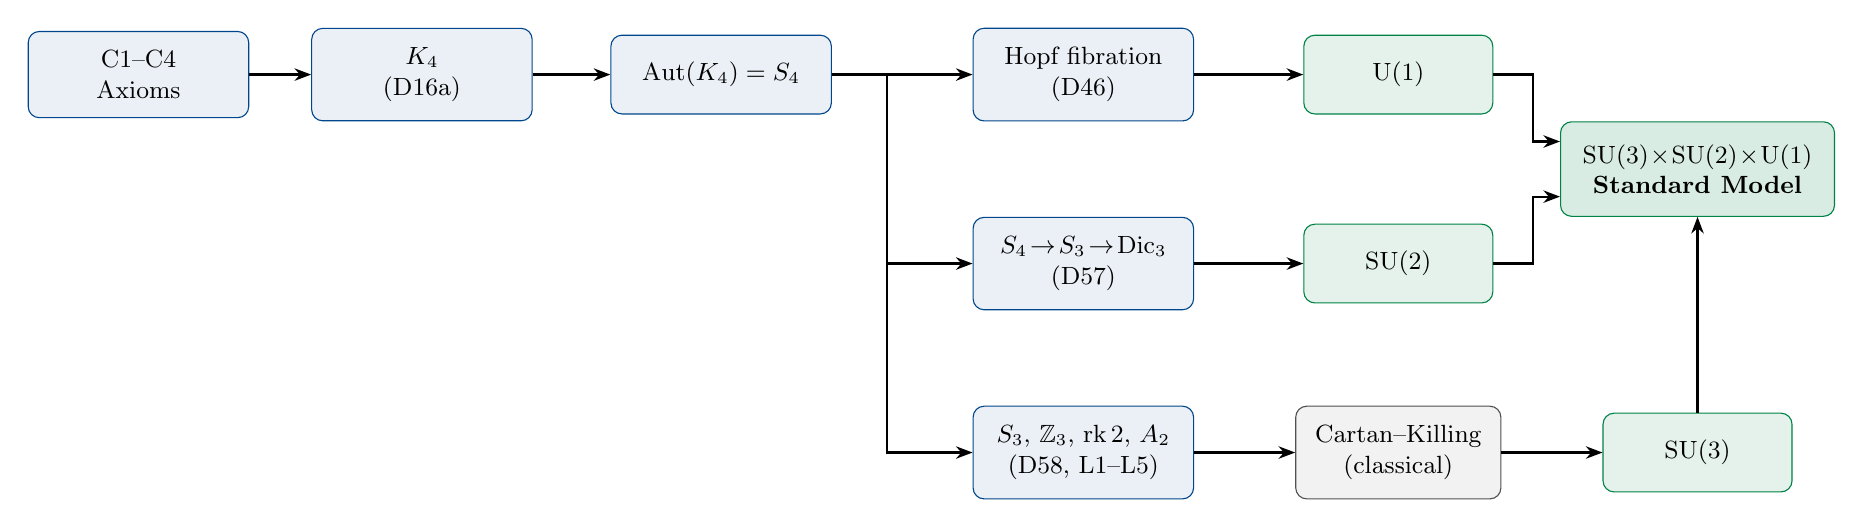
\begin{tikzpicture}[
  every node/.style={font=\small},
  pnode/.style={
    draw=proofblue, fill=proofblue!8,
    rounded corners=4pt, align=center,
    inner sep=7pt, minimum width=2.8cm, minimum height=1.0cm
  },
  gnode/.style={
    draw=resolvedgreen, fill=resolvedgreen!10,
    rounded corners=4pt, align=center,
    inner sep=7pt, minimum width=2.4cm, minimum height=1.0cm
  },
  cnode/.style={
    draw=darkgray, fill=gray!10,
    rounded corners=4pt, align=center,
    inner sep=7pt, minimum width=2.6cm, minimum height=1.0cm
  },
  smnode/.style={
    draw=resolvedgreen, fill=resolvedgreen!15,
    rounded corners=4pt, align=center,
    inner sep=8pt, minimum width=3.4cm, minimum height=1.2cm,
    font=\small\bfseries
  },
  arr/.style={-{Stealth[length=6pt]}, thick}
]

\node[pnode] (C1C4) at (0, 0) {C1--C4\\Axioms};
\node[pnode] (K4)   at (3.6, 0) {$K_4$\\(D16a)};
\node[pnode] (AUT)  at (7.4, 0) {$\mathrm{Aut}(K_4)=S_4$};

\node[pnode] (HOPF) at (12.0,  0.0) {Hopf fibration\\(D46)};
\node[pnode] (DIC3) at (12.0, -2.4) {$S_4\!\to\!S_3\!\to\!\mathrm{Dic}_3$\\(D57)};
\node[pnode] (L1L5) at (12.0, -4.8) {$S_3,\,\mathbb{Z}_3,\,\mathrm{rk}\,2,\,A_2$\\(D58, L1--L5)};

\node[gnode] (U1)  at (16.0,  0.0) {$\mathrm{U}(1)$};
\node[gnode] (SU2) at (16.0, -2.4) {$\mathrm{SU}(2)$};
\node[cnode] (CK)  at (16.0, -4.8) {Cartan--Killing\\(classical)};

\node[gnode] (SU3) at (19.8, -4.8) {$\mathrm{SU}(3)$};

\node[smnode] (SM) at (19.8, -1.2)
  {$\mathrm{SU}(3)\!\times\!\mathrm{SU}(2)\!\times\!\mathrm{U}(1)$\\Standard Model};

%% Axe horizontal
\draw[arr] (C1C4) -- (K4);
\draw[arr] (K4)   -- (AUT);

%% De AUT : horizontal vers HOPF, coudes vers DIC3 et L1L5
\draw[arr] (AUT.east) -- (HOPF.west);
\draw[arr] (AUT.east) -- ++(0.7,0) |- (DIC3.west);
\draw[arr] (AUT.east) -- ++(0.7,0) |- (L1L5.west);

%% Dérivations vers groupes de jauge
\draw[arr] (HOPF)  -- (U1);
\draw[arr] (DIC3)  -- (SU2);
\draw[arr] (L1L5)  -- (CK);
\draw[arr] (CK)    -- (SU3);

%% U(1) et SU(2) vers SM (entrée par la gauche)
\draw[arr] (U1.east)  -- ++(0.5,0) |- ([yshift= 0.35cm]SM.west);
\draw[arr] (SU2.east) -- ++(0.5,0) |- ([yshift=-0.35cm]SM.west);

%% SU(3) vers SM (entrée par le bas)
\draw[arr] (SU3.north) -- ++(0,0.55) -| (SM.south);

\end{tikzpicture}%
}
\caption{The complete causal chain from the \PDL\ axioms C1--C4 to the Standard Model gauge group $\SUthree \times \SUtwo \times \Uone$. Blue boxes denote \PDL\ theorems; the grey box denotes the classical Cartan--Killing--Weyl classification taken as established mathematical apparatus; green boxes denote the three gauge factors. The chain for $\SUthree$ (this document) closes the algebraic derivation of the Standard Model gauge group.}
\label{fig:gauge_group_chain}
\end{figure}

\subsection{What this corollary does and does not assert}

It is essential to be precise about the scope of Corollary~\ref{cor:SM_gauge_group}. What is established:
\begin{itemize}[leftmargin=2em]
\item The \emph{algebraic structure} of the Standard Model gauge group as a product of three compact simple Lie groups.
\item The specific identification of each factor as $\SUthree$, $\SUtwo$, $\Uone$ (not $\PSUthree$, not $\mathrm{SO}(3)$, not $\mathrm{U}(2)$, etc.).
\item The chain of structural lemmas from C1--C4 to each factor.
\end{itemize}
What is \emph{not} established by Corollary~\ref{cor:SM_gauge_group}:
\begin{itemize}[leftmargin=2em]
\item The \emph{physical identification} of $\SUthree$ with $\SUthree_{\mathrm{c}}$ acting on the proton triplet $(u,u,d)$ in the fundamental representation $\mathbf{3}$. This is Open Problem $\mathrm{OP\text{-}D58\text{-}1}$ (Section~\ref{sec:openproblems}).
\item The \emph{representation content} of fermions under each gauge factor, including their electric charges, hypercharges, and weak isospins.
\item The \emph{three generations} of fermions.
\item The \emph{mass spectrum}, the Higgs mechanism, the CKM and PMNS mixing matrices.
\end{itemize}
These remain genuine open problems of the programme. The corollary establishes the algebraic skeleton; the phenomenological flesh is the task of future documents.

% ============================================================
\section{Documented negative result: \texorpdfstring{$\Vfour$}{V4} on \texorpdfstring{$H_1(\Kfour;\RR)$}{H1(K4;R)}}
\label{sec:negative}

\subsection{The natural but failed strategy}

A natural strategy, examined and discarded during the development of D58, would have been to identify the three-element set on which $\Sthree = \Sfour/\Vfour$ acts with the basis of the first homology group $H_1(\Kfour;\RR)$. This is geometrically appealing because $\beta_1(\Kfour) = 3$, the dimension of $H_1(\Kfour;\RR)$, matches the three cycles needed to generate the cyclomatic structure of $\Kfour$. The hope would be that $\Vfour$ acts trivially on $H_1(\Kfour;\RR)$, leaving an effective $\Sthree$ action.

\subsection{Why the strategy fails}

\begin{proposition}[Faithfulness of $\Sfour$ on $H_1(\Kfour;\RR)$]
\label{prop:negative}
The induced action of $\Sfour = \Aut(\Kfour)$ on the cycle homology $H_1(\Kfour;\RR)$ is faithful: the kernel of the action $\Sfour \to \GL(H_1(\Kfour;\RR))$ is trivial. In particular, the Klein four-group $\Vfour$ acts non-trivially on $H_1(\Kfour;\RR)$; each of its three non-identity elements is represented by a distinct, non-identity, integer matrix in any cycle basis.
\end{proposition}

\begin{proof}
As a representation of $\Sfour$, the cycle homology $H_1(\Kfour;\RR)$ has dimension $\beta_1(\Kfour) = 3$. It can be computed directly: the four triangles $T_k$ (each obtained by removing one of the four vertices) span a 4-dimensional space, subject to the single linear relation $T_0 - T_1 + T_2 - T_3 = 0$ (verified by direct computation, see the script). Hence $\dim H_1 = 4 - 1 = 3$.

The $\Sfour$-action on the four triangles is the permutation action on the four vertices (since $T_k$ is the triangle opposite vertex $k$, and permuting vertices permutes triangles). The 4-dimensional permutation representation of $\Sfour$ on $\RR^4$ decomposes as the trivial representation plus the standard 3-dimensional irreducible representation~\cite{Fulton_Harris}. The relation $T_0 - T_1 + T_2 - T_3 = 0$ generates the kernel of the projection to the standard rep, hence the quotient $H_1(\Kfour;\RR)$ is isomorphic to the standard 3-dimensional irreducible representation of $\Sfour$.

The standard 3-dimensional irreducible representation of $\Sfour$ is faithful: its kernel is the trivial subgroup~\cite{Fulton_Harris}. Hence the $\Sfour$-action on $H_1(\Kfour;\RR)$ is faithful, and in particular $\Vfour$ acts non-trivially.

The verification script confirms this explicitly: for each non-identity element of $\Vfour$, the matrix in a cycle basis is computed explicitly and shown to be non-identity. The three matrices are:
\begin{align*}
(0,1)(2,3) &\;\longmapsto\; \begin{pmatrix} -1 & 0 & 0 \\ 1 & 0 & -1 \\ -1 & -1 & 0 \end{pmatrix},\\
(0,2)(1,3) &\;\longmapsto\; \begin{pmatrix} 0 & 1 & 1 \\ 0 & -1 & 0 \\ 1 & 1 & 0 \end{pmatrix},\\
(0,3)(1,2) &\;\longmapsto\; \begin{pmatrix} 0 & -1 & -1 \\ -1 & 0 & 1 \\ 0 & 0 & -1 \end{pmatrix},
\end{align*}
in the cycle basis $(T_1, T_2, T_3)$. None equals the identity.\qed
\end{proof}

\subsection{Consequence: the natural object is \texorpdfstring{$\Vfour \setminus \{e\}$}{V4 minus e}, not \texorpdfstring{$H_1$}{H1}}

The negative result of Proposition~\ref{prop:negative} clarifies the importance of Lemma~L2: the natural three-element set on which $\Sthree = \Sfour/\Vfour$ acts cannot be the cycle homology $H_1(\Kfour;\RR)$ (which is the faithful standard representation of $\Sfour$, hence \emph{does not} descend to a representation of the quotient). Instead, the correct natural set is $\Vfour \setminus \{e\}$, equivalently the three $\Vfour$-orbits on the six edges of $\Kfour$, equivalently the three partitions of $\{0,1,2,3\}$ into two unordered pairs --- the readings of Table~\ref{tab:three_readings}.

This negative result is documented here both for transparency (the development of D58 began with the hypothesis that the natural object would be $H_1$, and was corrected after script verification) and for guidance (any future extension of the gauge derivation should respect the same constraint: the relevant $\Sthree$-set is associated with $\Vfour \setminus \{e\}$, not with the cycle homology).

% ============================================================
\section{Computational verification}
\label{sec:verification}

\subsection{Supplementary script}

The full derivation of D58 is accompanied by the verification script
\begin{center}
\texttt{PDL\_SU3\_script1.py}~\cite{PDL_SU3_script1},
\end{center}
which provides exhaustive computational verification of every lemma using exact integer arithmetic. The script is self-contained and depends only on the standard library, \texttt{numpy}, and \texttt{networkx}, executing in seconds on any modern Python 3 environment.

\subsection{Scope of the verification}

The script verifies the following items, each by exhaustive enumeration over the relevant finite group or finite set:

\begin{table}[H]
\centering
\caption{Items verified by \texttt{PDL\_SU3\_script1.py}.}
\label{tab:verification}
\renewcommand{\arraystretch}{1.25}
\small
\begin{tabular}{p{4.7cm} p{7.0cm} l}
\toprule
\textbf{Verification} & \textbf{Method} & \textbf{Status} \\
\midrule
$\beta_1(\Kfour) = 3$ & \texttt{networkx} cyclomatic count & PASSED \\
$|\Sfour|$, $|\Afour|$, $|\Vfour|$ counts & Direct enumeration & PASSED \\
$\Vfour$ normal in $\Sfour$ & Exhaustive conjugation, 96 cases & PASSED \\
L1: $\Sfour/\Vfour$ non-abelian & Coset multiplication table & PASSED \\
L2(a)(b): $\rho$ surjective, $\ker\rho = \Vfour$ & Conjugation on $\Vfour\setminus\{e\}$, 24 cases & PASSED \\
L2(c): 3 orbits + $\Sfour$-equivariance & Exhaustive on 24 elements & PASSED \\
L3: $\Afour/\Vfour \cong \Zthree$ & Direct enumeration over $\Afour$ & PASSED \\
L4: trivial + standard $\Sthree$-invariant & 6 matrices on test vectors & PASSED \\
L5: 6 roots of length $\sqrt{2}$ form $A_2$ & Inner-product computation & PASSED \\
Negative: $\Vfour$ non-trivial on $H_1$ & Explicit matrices in cycle basis & VERIFIED NEG. \\
\bottomrule
\end{tabular}
\end{table}

\subsection{Reproducibility}

The script is deterministic and uses no random sampling. The output is bit-for-bit reproducible across platforms. A reference output file \texttt{PDL\_SU3\_script1\_output.txt} is provided alongside the script for line-by-line comparison.

\subsection{The \PDL\ verrouillage protocol}

In accordance with the \PDL\ verrouillage protocol (established for the corpus and used uniformly since D29), no claim of D58 was incorporated into this document before independent execution of the verification script. The five lemmas were verrouillés (locked) by independent Colab execution before LaTeX drafting began.

% ============================================================
\section{Open problems}
\label{sec:openproblems}

\subsection{The natural successors to D58}

D58 closes the algebraic derivation of the Standard Model gauge group. It opens a small number of well-defined problems whose resolution would further the programme.

\begin{openproblem}[OP-D58-1 --- Physical identification of $\SUthree$ with $\SUthree_{\mathrm{c}}$]
\label{op:D58-1}
Identify, within the \PDL\ formalism, the explicit map between the algebraic $\SUthree$ derived in this document and the physical colour gauge group $\SUthree_{\mathrm{c}}$ of quantum chromodynamics. Specifically, construct the fundamental representation $\mathbf{3}$ of $\SUthree$ as an action on a 3-dimensional space identified with one of the candidate triplets associated with $\Kfour$:
\begin{itemize}[leftmargin=2em]
\item the proton triplet $(u,u,d)$ (via D47~\cite{PDL_D47});
\item the three leakage cycles with prime exponents $(p_{k_1}, p_{k_2}, p_{k_3}) = (23, 67, 997)$ (via D51~\cite{PDL_D51} and D52~\cite{PDL_D52});
\item the three $\Vfour$-orbits on edges, equivalently $\Vfour \setminus \{e\}$ (the present document, Lemma~L2).
\end{itemize}
The first identification (with the proton triplet $(u,u,d)$) is the goal closest to standard QCD; the third (with the $\Vfour$-orbits) is closest to the structural source of $\SUthree$ derived here. The compatibility of these three identifications, or the establishment of a canonical map between them, is the content of OP-D58-1. \textbf{Priority:} high. \textbf{Entry points:} D47, D51, D52, D58 (Lemma~L2).
\end{openproblem}

\begin{openproblem}[OP-D58-2 --- The three triplets associated with $\Kfour$]
\label{op:D58-2}
Establish formally the relationship between the three triplets identified in Remark~\ref{rem:three_triplets}:
\begin{enumerate}[label=(T\arabic*),leftmargin=2em]
\item the three independent cycles in $H_1(\Kfour;\ZZ)$ (D51);
\item the three leakage cycles with prime exponents $(23, 67, 997)$ (D51, D52);
\item the three $\Vfour$-orbits on edges, equivalently $\Vfour \setminus \{e\}$ (D58, Lemma~L2).
\end{enumerate}
Are these triplets in canonical $\Sfour$-equivariant bijection? If so, what is the explicit map? If not, what is the precise nature of their relationship? Note that triplets~(T1) and~(T3) live in different representations of $\Sfour$ (the standard 3-dimensional irreducible for~(T1), the permutation representation pulled back from $\Sthree$ for~(T3)), so a naive bijection is excluded by Proposition~\ref{prop:negative}. \textbf{Priority:} medium. \textbf{Entry points:} D51, D52, D58.
\end{openproblem}

\begin{openproblem}[OP-D58-3 --- Fundamental representation of $\SUthree$ from C1--C4]
\label{op:D58-3}
The Lie algebra $\suthree$ has two inequivalent fundamental representations $\mathbf{3}$ and $\bar{\mathbf{3}}$ of dimension 3. In quantum chromodynamics, $\mathbf{3}$ acts on quarks and $\bar{\mathbf{3}}$ on antiquarks. Derive from C1--C4 the action of $\SUthree$ on a 3-dimensional complex space, and identify which of $\mathbf{3}$ or $\bar{\mathbf{3}}$ corresponds to the matter/antimatter distinction of the \PDL\ formalism. The asymmetry $\Delta n = n_d - n_u = 4$ (D47, theorem) may provide the structural origin of the matter--antimatter distinction. \textbf{Priority:} medium. \textbf{Entry points:} D47, D51, D58.
\end{openproblem}

\subsection{Connection to existing open problems}

D58 partially resolves the following open problems of the corpus:

\begin{resolvedproblem}[OP-D57-3 / OP-SU3 --- $\SUthree$ from the proton hierarchy]
\textcolor{proofblue}{Algebraic part resolved by D58.} The algebraic derivation of $\SUthree$ from C1--C4 is the content of Theorem~\ref{thm:D58_main} of the present document. The physical identification with $\SUthree_{\mathrm{c}}$ acting on $(u,u,d)$ remains open as OP-D58-1.
\end{resolvedproblem}

\begin{resolvedproblem}[OP-OFN-1 (partial) --- $\beta_1 = 3$ as a shared invariant]
\textcolor{proofblue}{Partial resolution from D57 reinforced by D58.} D57 established $\Afour/\Vfour \cong \Zthree$ as the algebraic origin of the integer 3 in both $\beta_1(\Kfour) = 3$ and $b_1(\Omega_{21}) = 3$~\cite{PDL_N01}. D58 extends this by establishing that the same $\Zthree = \Afour/\Vfour$ is the centre of $\SUthree$ in the \PDL\ derivation. The formal correspondence between the three \PDL\ leakage cycles and the three OFN fermion generations remains open.
\end{resolvedproblem}

% ============================================================
\section{Epistemic status table}
\label{sec:epistemic}

Table~\ref{tab:epistemic_D58} gives the complete epistemic stratification of all claims of D58.

\begin{table}[H]
\centering
\caption{Complete epistemic stratification of D58 claims.}
\label{tab:epistemic_D58}
\renewcommand{\arraystretch}{1.3}
\begin{tabular}{p{6.5cm} p{3cm} p{4.5cm}}
\toprule
\textbf{Claim} & \textbf{Status} & \textbf{Source} \\
\midrule
$\Kfour$ minimal admissible closure & Theorem (C1--C4) & D16a~\cite{PDL_D16a} \\
$\Re = |E(\Kfour)| = 6$ & Theorem (C1--C4) & D16a~\cite{PDL_D16a} \\
$\Vfour$ normal in $\Sfour$ & Theorem (group theory) & Lemma~\ref{lem:L1} \\
$\Sfour/\Vfour \cong \Sthree$ (Lemma L1) & Theorem (group theory) & Lemma~\ref{lem:L1} \\
$\Aut(\Vfour) \cong \Sthree$ & Theorem (group theory) & Lemma~\ref{lem:L2}(a) \\
$\rho\colon \Sfour \to \Sthree$ surjective, kernel $\Vfour$ & Theorem (group theory) & Lemma~\ref{lem:L2}(b) \\
$S_4$-equivariant bijection $\Vfour\setminus\{e\} \leftrightarrow$ orbits & Theorem (C1--C4) & Lemma~\ref{lem:L2}(c) \\
$\Afour/\Vfour \cong \Zthree$ (Lemma L3) & Theorem (group theory) & Lemma~\ref{lem:L3} \\
Rank-2 Cartan from $\Re = 6$ (Lemma L4) & Theorem (C1--C4) & Lemma~\ref{lem:L4} \\
$A_2$ root system (Lemma L5) & Theorem (root systems) & Lemma~\ref{lem:L5} \\
\textbf{$\SUthree$ from C1--C4 (main theorem)} & \textbf{Theorem} (classical) & \textbf{Theorem~\ref{thm:D58_main}} \\
$\SUthree \times \SUtwo \times \Uone$ algebraic & Corollary & Cor.~\ref{cor:SM_gauge_group} \\
$\Vfour$ non-trivial on $H_1(\Kfour;\RR)$ & Theorem (verified) & Prop.~\ref{prop:negative} \\
Physical id.\ with $\SUthree_{\mathrm{c}}$ & Open problem & OP-D58-1 \\
Bijection among three triplets & Open problem & OP-D58-2 \\
Fundamental rep.\ $\mathbf{3}$ from C1--C4 & Open problem & OP-D58-3 \\
\bottomrule
\end{tabular}
\end{table}

The label ``Theorem (classical)'' for the main theorem indicates that its proof invokes the Cartan--Killing--Weyl classification, a universally accepted result of mathematics, which is not re-proved in this document. The label ``Theorem (group theory)'' indicates that the proof is purely group-theoretic and could in principle be reconstructed from first principles using standard texts~\cite{Rotman_Groups}. The label ``Theorem (C1--C4)'' indicates that the proof additionally invokes specific structural results of the \PDL\ corpus.

% ============================================================
\section{Conclusion and outlook}
\label{sec:conclusion}

\subsection{What D58 achieves}

D58 closes the algebraic derivation of the Standard Model gauge group within the \PDL\ programme. Combined with D46 ($\Uone$) and D57 ($\SUtwo$), the structure $\SUthree \times \SUtwo \times \Uone$ is now an unconditional theorem of C1--C4 (modulo classical Cartan--Killing--Weyl theory). The derivation rests on five lemmas, all verifiable by exhaustive integer computation, with no free parameters and no auxiliary hypotheses beyond the four axioms of the programme.

The key structural identification of D58 is Lemma~L2: the natural three-element set on which $\Sthree = \Sfour/\Vfour$ acts is the set $\Vfour \setminus \{e\}$, equivalently the three $\Vfour$-orbits on the six edges of $\Kfour$. This identification is the result of a corrected strategy: the script verification revealed that the alternative identification with the cycle homology $H_1(\Kfour;\RR)$ fails because $\Vfour$ acts faithfully on $H_1$ (Section~\ref{sec:negative}). The corrected strategy succeeds in all five lemmas.

\subsection{What D58 does not achieve}

The honest stratification of claims (Section~\ref{sec:epistemic}) makes clear what D58 does not establish:
\begin{itemize}[leftmargin=2em]
\item The physical identification of the derived $\SUthree$ with the colour gauge group $\SUthree_{\mathrm{c}}$ of QCD acting on quark triplets.
\item The fundamental representation $\mathbf{3}$ and antifundamental $\bar{\mathbf{3}}$ as explicit constructions from C1--C4.
\item The three generations of fermions, their masses, the CKM and PMNS mixing matrices.
\item The Higgs mechanism and the spontaneous breaking $\SUtwo \times \Uone \to \Uone_{\mathrm{em}}$.
\end{itemize}
These remain genuine open problems of the programme. Their solution would not invalidate D58, but would deepen the gauge structure beyond its purely algebraic skeleton.

\subsection{Position in the wider literature}

The derivation of the Standard Model gauge group from first principles has been a long-standing problem of theoretical physics. The major existing programmes ---- grand unification, string theory, noncommutative geometry, and several others --- have at best derived the algebraic structure of the group, without the complete fermionic content. The \PDL\ derivation of D46+D57+D58 places the gauge group structure on the same epistemic footing: established as an algebraic theorem from a minimal set of axioms, with the phenomenological content remaining as a future task.

What distinguishes the \PDL\ derivation is the economy of its starting point: four combinatorial axioms on finite signed graphs, with no presupposed space--time, no continuum, no field content. The derivation reaches the gauge group structure through algebra and finite combinatorics only. This austerity is at once a strength (no hidden assumptions) and a limitation (no continuous structure to draw fermionic representations from). The forthcoming work to address OP-D58-1, OP-D58-2, OP-D58-3 will reveal whether this austerity can be extended to the representation content or whether further structural input is required.

\subsection{Next steps}

The immediate next documents in the \PDL\ programme are:
\begin{enumerate}[leftmargin=2em]
\item \textbf{Document D59} (forthcoming): construction of the fundamental representation $\mathbf{3}$ of $\SUthree$ as an action on a 3-dimensional space identified with the three leakage cycles of D51/D52, addressing OP-D58-1 and OP-D58-3. Requires computational verification of compatibility with C4.
\item \textbf{Document D-electroweak-WZ}: derivation of the $W/Z$ mass ratio $M_W/M_Z = \cos(19\pi/119)$ as a parameter-free prediction (OP10-c of the global mapping~\cite{PDL_DM}), now actionable given the gauge group structure.
\item \textbf{Joint document with Evdokimov}: the present results sharpen the partial resolution of OP-OFN-1; the joint document ``Three Roads to the Periodic Table''~\cite{Evdokimov_TwoRoads} will incorporate D58 in its revised version.
\end{enumerate}

\subsection{Final remark}

The completion of the gauge group derivation is a structural milestone of the \PDL\ programme but should be understood in proportion: it is not a derivation of the Standard Model, only of its algebraic skeleton. The phenomenological content of the Standard Model --- fermion masses, mixing angles, three generations --- remains as challenging in \PDL\ as in any other programme. The contribution of D58 is to put the algebraic gauge group structure on the same axiomatic footing as the other major results of the corpus, in the spirit of Hilbert's call for the axiomatic derivation of physics from minimal foundations.

% ============================================================
\section*{Acknowledgements}

The author thanks Oleg~I.~Evdokimov for the identification of $\Afour/\Vfour \cong \Zthree$ in the joint document on the convergence between the \PDL\ and OFN frameworks~\cite{Evdokimov_TwoRoads}, which provided one of the structural ingredients of the present derivation. The author also thanks the colleagues at ResearchGate who responded to Question~Q2 on the combinatorial derivation of fundamental physical constants and gauge groups; their critical engagement helped sharpen the formulation of the open problems identified here.

\vspace{0.5em}

All scripts, results, and source files are available at:
\begin{center}
\url{https://github.com/laubscher-lab/PDL-framework}
\end{center}

% ============================================================
\clearpage
\bibliographystyle{unsrt}
\bibliography{D58_references}
% ============================================================

\end{document}